\documentclass[a4paper, 12pt]{article}%тип документа

%отступы
\usepackage[left=2cm,right=2cm,top=2cm,bottom=3cm,bindingoffset=0cm]{geometry}

%Русский язык
\usepackage[T2A]{fontenc} %кодировка
\usepackage[utf8]{inputenc} %кодировка исходного кода
\usepackage[english,russian]{babel} %локализация и переносы

%Вставка картинок
\usepackage{wrapfig}
\usepackage{graphicx}
\graphicspath{{pictures/}}
\DeclareGraphicsExtensions{.pdf,.png,.jpg}

%оглавление
\usepackage{titlesec}
\titlespacing{\chapter}{0pt}{-30pt}{12pt}
\titlespacing{\section}{\parindent}{5mm}{5mm}
\titlespacing{\subsection}{\parindent}{5mm}{5mm}
\usepackage{setspace}

%Графики
\usepackage{multirow}
\usepackage{pgfplots}
\pgfplotsset{compat=1.9}

%Математика
\usepackage{amsmath, amsfonts, amssymb, amsthm, mathtools}

%Стиль страницы
\usepackage{fancyhdr}
\pagestyle{fancy}

\begin{document}

\begin{titlepage}

\begin{center}
%\vspace*{1cm}
\large\textbf{Московский Физико-Технический Институт}\\
\large\textbf{(национальный исследовательский университет)}
\vfill
\line(1,0){430}\\[3mm]
\huge\textbf{Лабораторная работа №4.4.4}\\
\large\textbf{Интерферометр Фабри-Перо}\\
\line(1,0){430}\\[1mm]
\vfill
\large Баканова К.В., Б01-003\\
%\vspace*{1cm}
\large февраль 2022 г.\\
\end{center}

\end{titlepage}




\section{Аннотация}
\fancyhead[L] {Лабораторная работа №4.4.4}
\fancyhead[R] {Баканова К.В.}
В данной работе проводится измерение длины волны жёлтых линий ртути, жёлтого дублета натрия, а также определение спектральных характеристик интерферометра Фабри—Перо. 


\section{Теоретические сведения}
\fancyhead[L] {Лабораторная работа №4.4.4}
\fancyhead[R] {Баканова К.В.}

Интерферометр Фабри–Перо состоит из двух стеклянных или кварцевых пластин с хорошо отполированными поверхностями. На одну поверхность каждой пластины нанесены отражающие свет покрытия. Интерферометр можно рассматривать как плоскопараллельную пластину, в которой происходят многократные отражения и интерференция световых волн (рис. \ref{fig:reflections}). 

		\begin{figure}[h!]
		\centering
	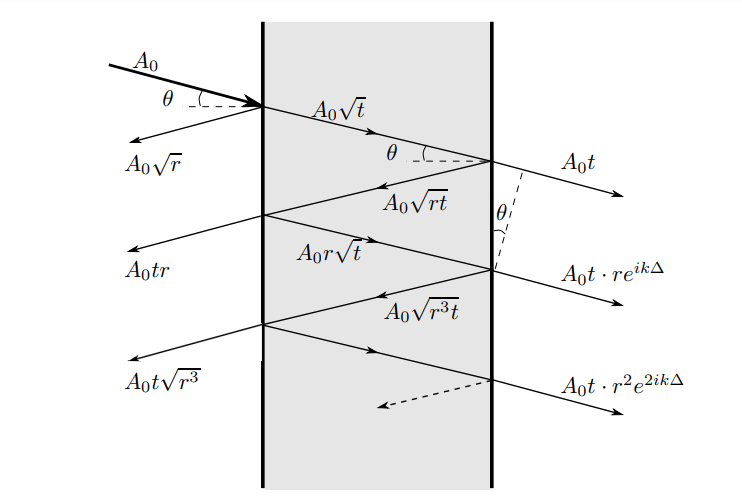
\includegraphics[width=0.6\linewidth]{Screenshot_1.png}
	\caption{Прохождение волны через интерферометр Фабри---Перо}
	\label{fig:reflections}
\end{figure}

Найдём условие возникновения интерференционной картины для световой волны с длиной $ \lambda $. Выразим разность хода двух интерферирующих волн, падающих на интерферометр под углом $ \theta $:

\begin{equation*}\label{key}
	\delta = 2 L \cos \theta,
\end{equation*}
где через $ \delta $ обозначена разность хода двух волн, а через $ L $ -- база интерферометра. Отсюда условие максимума интенсивности интерферирующих волн:
\begin{equation*}\label{key}
	2 L \cos \theta_m = m \lambda.
\end{equation*}
Оно же является условием резонанса, при выполнении которого интерферометр просветляется для данной длины волны $ \lambda $.

		\begin{figure}[h!]
		\centering
		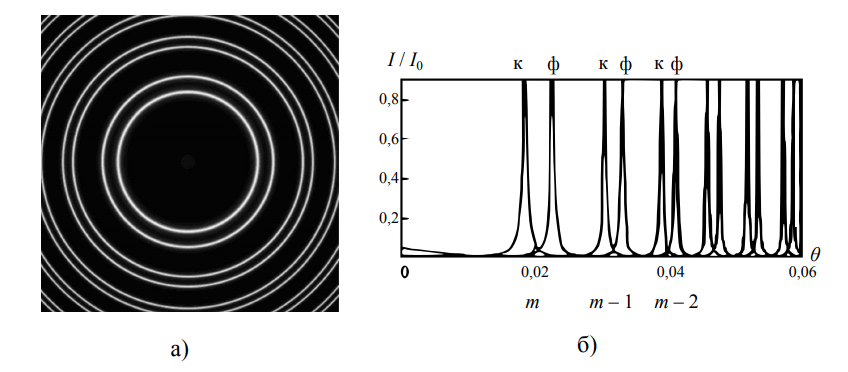
\includegraphics[width=0.7\linewidth]{Screenshot_2.png}
		\caption{а) Наблюдаемая интерференционная картина; б) Зависимость интенсивности света от угла $ \theta $}
		\label{fig:screenshot2}
	\end{figure}

Для малых углов и больших порядков спектра угловая дисперсия определяется соотношением:
\begin{equation*}\label{key}
	D = \frac{d \theta}{d \lambda} = - \frac{m}{2 m \sin \theta_m} \approx - \frac{1}{\lambda \theta_m}.
\end{equation*}

Разрешающая способность для порядка спектра $ m \approx \frac{2 L}{\lambda} $:
\begin{equation*}\label{key}
	R = \frac{\lambda}{\Delta \lambda}= \frac{\pi\sqrt{r} m }{(1-r)}
\end{equation*}





	\subsection{Натриевая лампа}
\fancyhead[L] {Лабораторная работа №4.4.4}
\fancyhead[R] {Баканова К.В.}

\item Схема экспериментальной установки представлена на рис. 1. Свет от ртутной лампы $ S $, пройдя через линзу Л$_0 $ и светофильтр $ C $, попадает на интерферометр Фабри-Перо (ИФП). Линза Л$_0 $ служит для формирования пучка лучей (слегка сходящегося или слегка расходящегося). Интерференционные кольца наблюдаются в локальной плоскости линзы Л. Картина рассматривается через зрительную трубу Т, сфокусированную на эту плоскость. Диаметры колец измеряются с помощью микроскопа катетометра.
\item    
		\begin{figure}[h!]
		\centering
		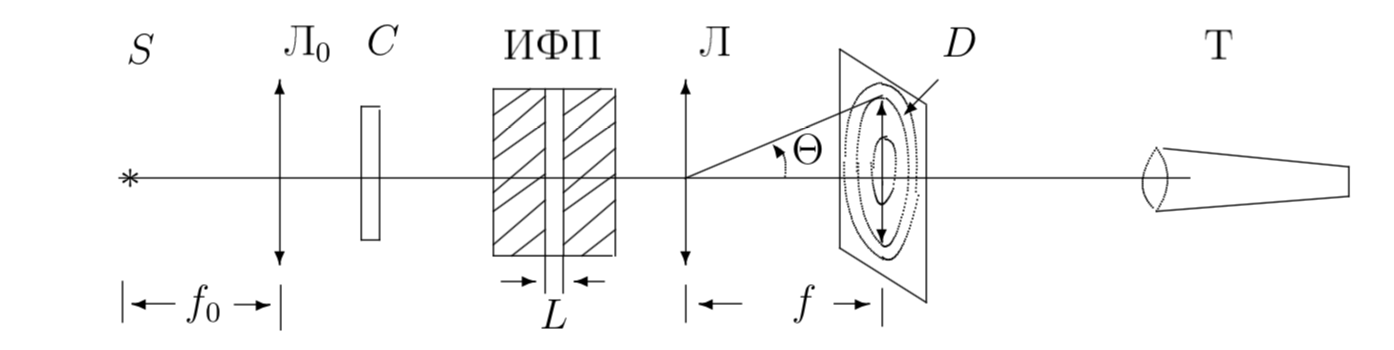
\includegraphics[width=\linewidth]{lab.png}
		\caption{Экспериментальная установка}
		\label{lab}
	\end{figure}

\item Зрительная труба $ Т $ и отсчетный микроскоп  --- элементы катетометра --- прибора, предназначенного для измерения расстояний в вертикальной плоскости вдоль вертикальной оси.  ртути состоит из нескольких компонентов. Расщепление этой спектральной линии связано с дополнительной энергией, возникающей как в результате взаимодействия магнитных моментов ядра и электрона --- \textit{сверхтонкая структура} (магнитное поле ядра действует на спиновый магнитный момент электрона), так и с \textit{изотопическим сдвигом} (в парах ртути присутствуют в заметных количествах изотопы с атомными массами от 198 до 204 а.е.м.). Каждое зелёное кольцо содержит более десятка близко расположенных компонентов, но разрешение нашего прибора не позволяет все их рассмотреть.
	Спектр натриевой лампы исследуется по аналогичной схеме, но светофильтр в этом случае не нужен, а интерферометр, линзы и зрительная труба катетометра
	имеют другие параметры.

\item    
\item    
		\section{Ход работы}
		\item    
		\subsection{Ртутная лампа}
		
\item После настройки интерферометра проведем измерения диаметров зеленых и желтых интерференционных колец с помощью катетометра, оценивая его погрешность измерения как $ \sigma_l = 0,3 $ мм. Параметр установки --- фокусное расстояние линзы $ f = 110 $ мм. Будем последовательно измерять расстояния $ l_1 $ от верхнего края 6-ого "<набора"> колец до нуля до центра, затем аналогично будем измерять расстояния $ l_2 $ от нижнего края до нуля. Результаты занесем в таблицы. 

			\begin{table}[h!]
			\caption{Измерение диаметров зеленых колец ртутной лампы}
			\begin{center}
				\begin{tabular}{|c|c|c|c|c|}
					\hline
					$ N $ & $ l_1 $, мм & $ l_2 $, мм & $ d_i^2 $, $ мм^2 $ & $ \sigma_d $, мм\\
					\hline
					 1 & 167.61 & 179.85 & 1.5 & 0.01 \\
					2 & 163.87 & 183.55 & 3.88 & 0.03 \\
					3 & 161.19 & 186.11 & 6.21 & 0.05 \\
					4 & 159.16 & 188.15 & 8.4 & 0.07 \\
					5 & 157.39 & 189.96 & 10.61 & 0.09 \\
					6 & 155.82 & 191.55 & 12.77 & 0.11 \\
					\hline
				\end{tabular}
			\end{center}
			\label{table}
		\end{table}
	
	\begin{table}[h!]
		\caption{Измерение диаметров желтых колец ртутной лампы}
		\begin{center}
			\begin{tabular}{|c|c|c|c|c|c|c|c|c|}
				\hline
					$ N $ & $ l_1 $, мм & $ l_2 $, мм & $ d $, мм & $ \overline{d} $,мм &  $ \sigma_d $,мм & $ \Delta d $, мм  &  $ 1/\Delta d $,$ мм^{-1} $ & $ \sigma_{1/\Delta d} $,$ мм^{-1} $\\
					\hline
			1 & 170.38 & 176.93 & 6.55 & 6.55 & 0.42 & 0 & - & - \\
			2 & 166.66 & 180.88 & 14.22 & 15.78 & 0.42 & 3.12 & 0.32 & 0.04 \\
			\text{} & 164.94 & 182.275 & 17.33 & \text{} & \text{} & \text{} & \text{} & \text{} \\
			
			3 & 162.94 & 184.27 & 21.33 & 22.31 & 0.42 & 1.97 & 0.51 & 0.08 \\
			\text{} & 161.995 & 185.295 & 23.3 & \text{} & \text{} & \text{} & \text{} & \text{} \\
			4 & 160.53 & 186.85 & 26.315 & 27.15 & 0.42 & 1.68 & 0.6 & 0.12 \\
			\text{} & 159.7 & 187.69 & 27.99 & \text{} & \text{} & \text{} & \text{} & \text{} \\
			5 & 158.36 & 188.95 & 30.585 & 30.96 & 0.42 & 1.35 & 0.74 & 0.18 \\
			\text{} & 157.69 & 189.03 & 31.34 & \text{} & \text{} & \text{} & \text{} & \text{} \\
			6 & 156.62 & 190.66 & 34.045 & 34.61 & 0.42 & 1.11 & 0.9 & 0.24 \\
			\text{} & 156.09 & 191.24 & 35.155 & \text{} & \text{} & \text{} & \text{} & \text{} \\
				\hline
			\end{tabular}
		\end{center}
		\label{table}
	\end{table}	

\item При этом погрешность $ \sigma_{1/\Delta d} $ мы оценивали как $ \sigma_{1/\Delta d} = \dfrac{\sigma_{\Delta d}}{\Delta d} \x \dfrac{1}{\Delta d} $.
	
\item Построим графики для зеленых и желтых колец:

		\begin{figure}[h!]
		\begin{center}
		\label{gr_graf}
		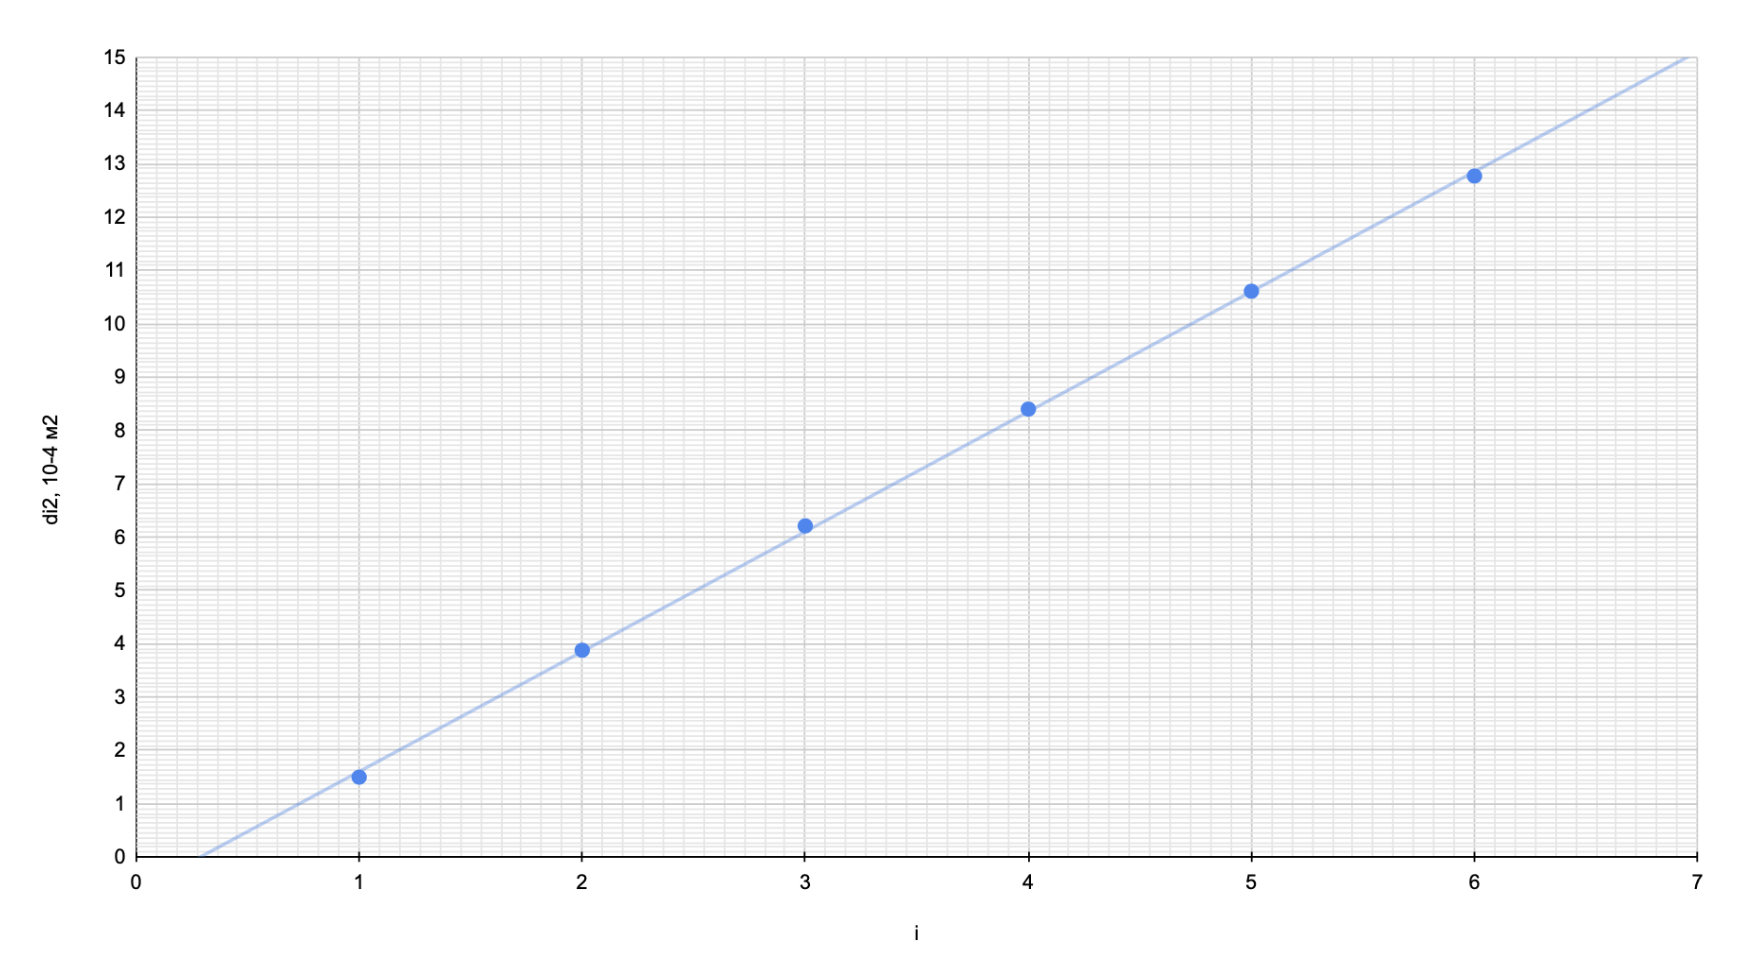
\includegraphics[scale=0.44]{green.png}
		\end{center}
		\caption{График зависимости $ d_i^2 $ от $ i $ зеленых линий $ Hg $}
	\end{figure}

\item Из полученных данных $ a = \dfrac{\varDelta (d_i^2)}{  \varDelta(i) } = (2,25 \pm 0,02) \x 10^{-4} $ м^2  \: \text{ рассчитаем базу L  интерферометра, взяв} $ \lambda(Hg) =  5461 $\AA :
	
	
	\begin{equation}\label{}
	\dfrac{\lambda}{L} = \dfrac{a}{4f^2}  \rightarrow 
	\te L =(0,117 \pm 0,001 ) \: \text{мм}
	\end{equation}
	
	\begin{figure}[h]
		\label{ye_graf}
		\begin{center}
		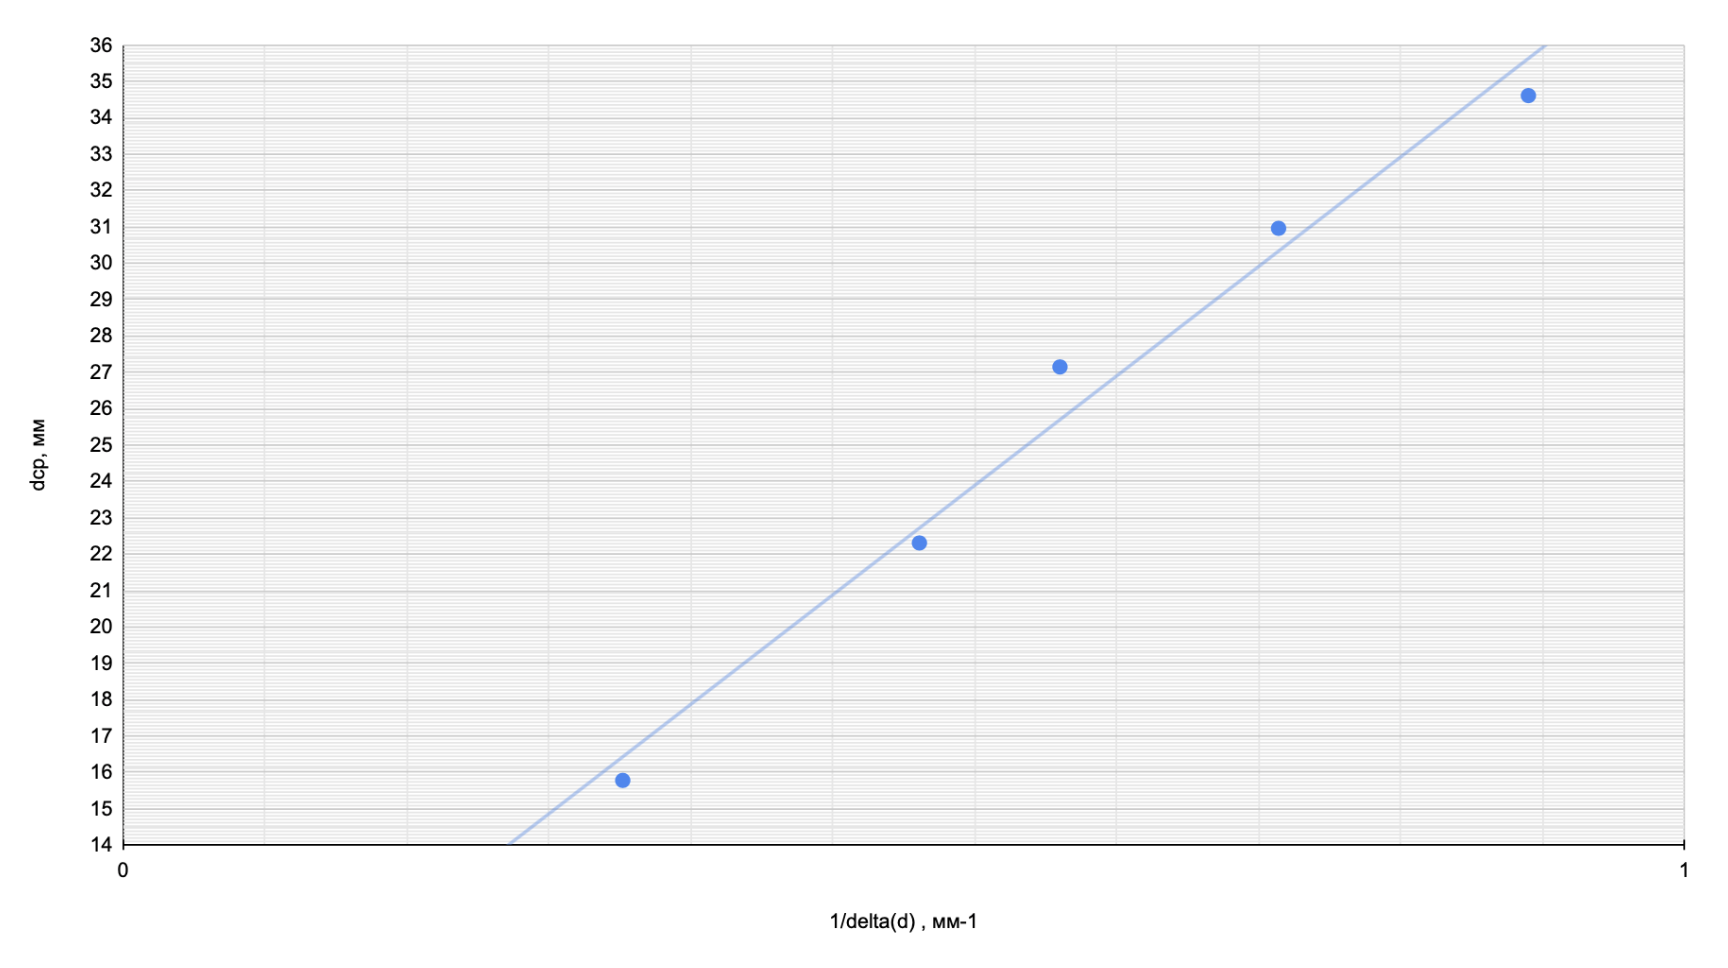
\includegraphics[scale=0.45]{yellow.png}
		\end{center}
		\caption{График зависимости $ \overline{d} $ от $ \dfrac{1}{\Delta d}$ желтых линий $ Hg $}
	\end{figure}

\item Из полученных данных $ a = \overline{d} \Delta d = (33,1 \pm 2,7) \x 10^{-6}$ м^2  \: \text{ рассчитаем разность длин волн} $ \Delta \lambda_р  $ 
  \: \text{интерферометра, взяв} $ \lambda(Hg) =  5780 $ \AA :
	
\[\Delta \lambda_=(\dfrac{\lambda a}{4f^2}) = (3,9 \pm 0,3) \text{\AA}\]
	

	\subsection{Натриевая лампа}
\fancyhead[L] {Лабораторная работа №4.4.4}
\fancyhead[R] {Баканова К.В.}

\item Проведем аналогичные измерения, сначала взяв одно из колец дублета ("<дальнее"> от центра), а затем для дублета. Фокусное расстояние $ f = 94 \; мм $. Результаты занесем в таблицу и построим графики.
	
	\begin{table}[h!]
		\caption{Измерение диаметров натриевых колец ртутной лампы}
		\begin{center}
			\begin{tabular}{|c|c|c|c|c|c|c|c|c|c|}
				\hline
				$ N $ & $ l_1 $, мм & $ l_2 $, мм & $ d $, мм  & $ d_i^2 $, $ мм^2 $ &$ \overline{d} $,мм &  $ \sigma_d $,мм & $ \Delta d $, мм  &  $ 1/\Delta d $,$ мм^{-1} $ & $ \sigma_{1/\Delta d} $,$ мм^{-1} $ \\
				\hline
				 1 & 148.89 & 140.49 & 8.4 & 0.71 & \text{--} & \text{} & - & \text{} & \text{} \\
				 2 & 152.29 & 137.27 & 15.03 & 2.26 & 16.14 & 0.59 & 2.22 & 0.45 & 0.05 \\
				 \text{} & 153.4 & 136.15 & 17.25 & \text{} & \text{} & \text{} & \text{} & \text{} & \text{} \\
				 3 & 155.29 & 134.13 & 21.16 & 4.48 & 21.97 & 0.59 & 1.61 & 0.62 & 0.07 \\
				 \text{} & 156.08 & 133.31 & 22.77 & \text{} & \text{} & \text{} & \text{} & \text{} & \text{} \\
				 4 & 157.62 & 131.77 & 25.85 & 6.68 & 26.46 & 0.59 & 1.22 & 0.82 & 0.09 \\
				 \text{} & 158.22 & 131.15 & 27.07 & \text{} & \text{} & \text{} & \text{} & \text{} & \text{} \\
				 5 & 159.61 & 129.85 & 29.76 & 8.86 & 30.33 & 0.59 & 1.13 & 0.88 & 0.12 \\
				 \text{} & 160.16 & 129.27 & 30.89 & \text{} & 0 & \text{} & \text{} & \text{} & \text{} \\
				 6 & 161.17 & 128.11 & 33.06 & 10.93 & 33.56 & 0.59 & 1.01 & 0.99 & 0.14 \\
				 \text{} & 161.71 & 127.65 & 34.07 & \text{} & \text{} & \text{} & \text{} & \text{} & \text{} \\
				\hline
			\end{tabular}
		\end{center}
		\label{Na2_table}
	\end{table}

	

	\begin{figure}[h!]
		\label{na1_graf}
				\begin{center}
		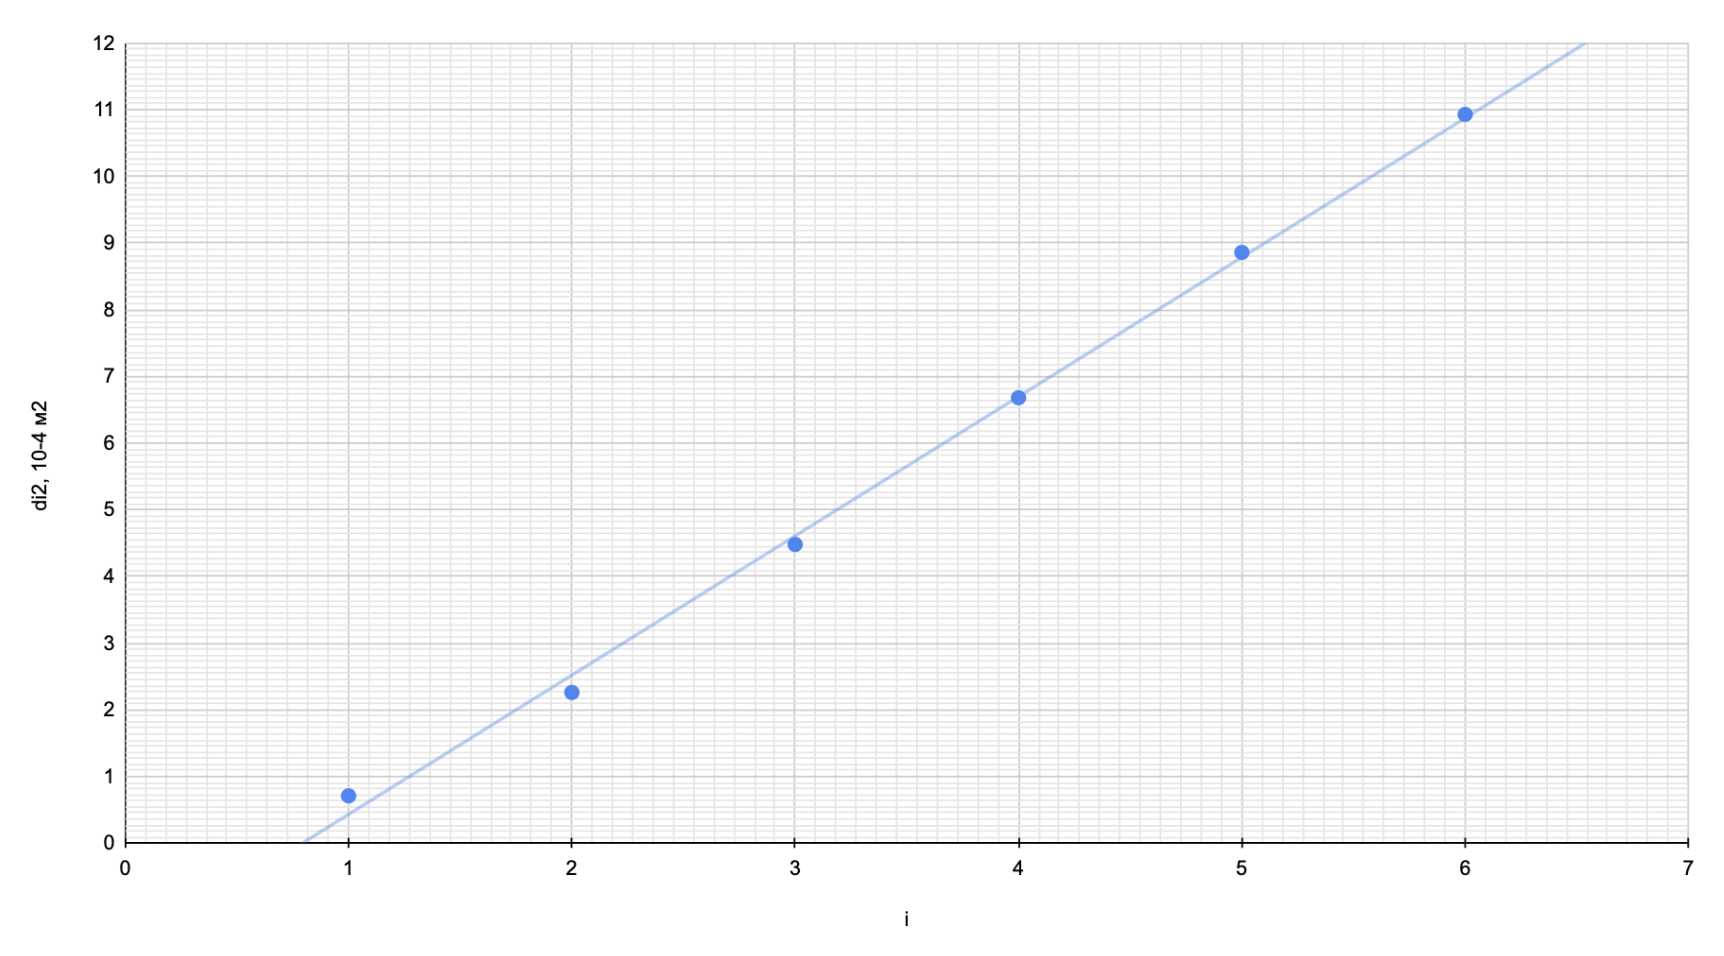
\includegraphics[scale=0.44]{na1.png}
				\end{center}
		\caption{График зависимости $ d_i^2 $ от $ i $ одной из линии дублета $ Na $}
	\end{figure}


\item Из полученных данных $ a = \dfrac{\varDelta (d_i^2)}{  \varDelta(i) } = (2,09 \pm 0,05) \x 10^{-4} $ м^2  \: \text{ рассчитаем базу L  интерферометра, взяв} $ \lambda(Hg) =  5893 $ \AA :


	\begin{equation}\label{}
	\dfrac{\lambda}{L} = \dfrac{a}{4f^2} \rightarrow 
	\te L = (0,100 \pm 0,002) \: \text{мм}
	\end{equation}

	
	\begin{figure}[h!]
		\label{na2_graf}
				\begin{center}
		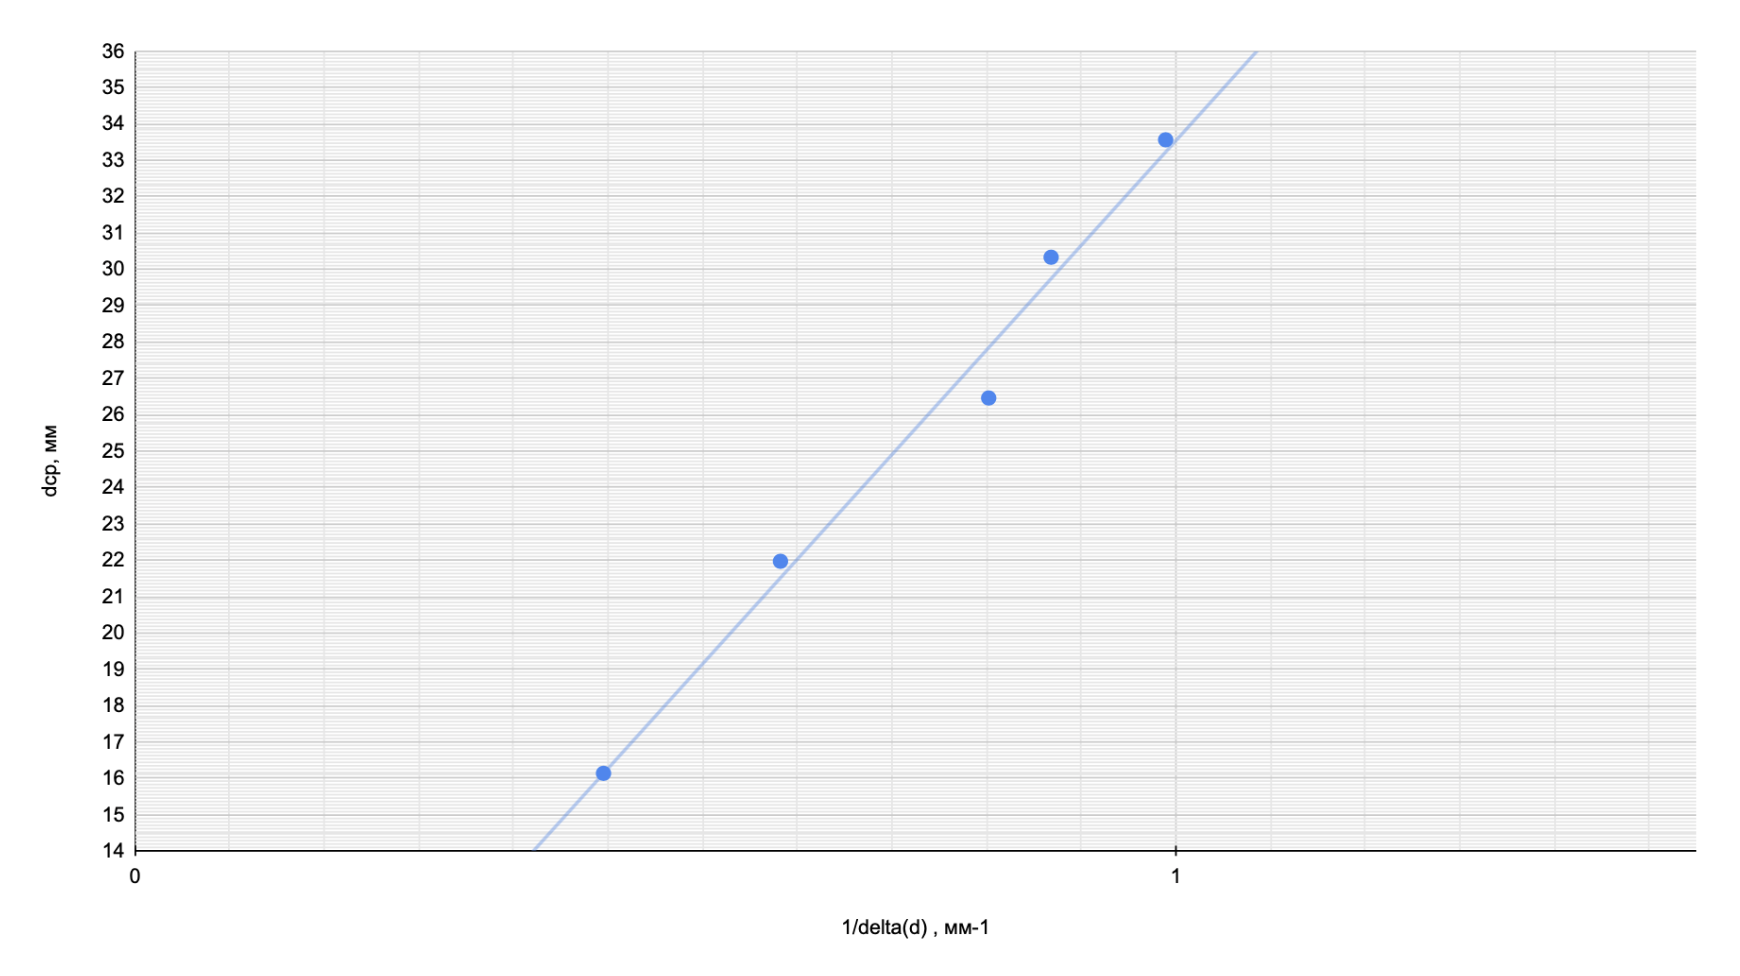
\includegraphics[scale=0.45]{na2.png}
		\end{center}
		\caption{График зависимости $ \overline{d} $ от $ \dfrac{1}{\Delta d}$ линий $ Na $}
	\end{figure}


\item Из полученных данных $ a = \overline{d} \Delta d = (33,6 \pm 2,1) \x 10^{-6} $ м^2  \: \text{ рассчитаем разность длин волн} $ \Delta \lambda_р  $ интерферометра, взяв $ \lambda(Hg) =  5893 $ \AA :

	\[\Delta \lambda = (\dfrac{\lambda a}{4f^2}) = (5,6 \pm 0,4) \text{\AA}\]

	\subsection{Дополнительные расчеты}
	
\item Сравним теоретические и экспериментальные значения линейной дисперсии интерферометра:
	
	\begin{table}[h!]
		\caption{Сравнение линейной дисперсии}
		\begin{center}
			\begin{tabular}{|c|c|c|c|c|c|c|c|c|}
				\hline
				$ \Delta d $, мм & $ D_э $, мм/\AA & 	$ \overline{d} $, мм & $ D_т $, мм/\AA  & $ <- Hg \; \; Na ->	 $&$ \Delta d $, мм & $ D_э $, мм/\AA & 	$ \overline{d} $, мм & $ D_т $, мм/\AA     \\
				\hline
			3.12 & 0.39 & 15.78 & 0.27 & & 2.22 & 0.2 & 16.14 & 0.19 \\
			1.97 & 0.25 & 22.32 & 0.19 & & 1.61 & 0.14 & 21.97 & 0.14 \\
			1.68 & 0.21 & 27.15 & 0.15 & & 1.22 & 0.11 & 26.46 & 0.11 \\
			1.35 & 0.17 & 30.96 & 0.14 & &1.13 & 0.1 & 30.33 & 0.1 \\
			1.11 & 0.14 & 34.6 & 0.12 & &1.01 & 0.09 & 33.56 & 0.09 \\
				\hline
			\end{tabular}
		\end{center}
		\label{}
	\end{table}
	Расчеты по формуле:
	\[D_e = \dfrac{\Delta d}{2 \Delta \lambda}, \quad D_t = \dfrac{2f^2}{\lambda \overline{d}}\]
	
	Рассчитаем аппаратную разрешающую способность:
	

	\[R_a = \dfrac{\lambda}{\delta \lambda} \backsimeq \dfrac{4f^2}{d \delta r}\]

	
	Для ртути $ R_a = 5,5 \x 10^{-3} $, для натрия $ R_a = 7,1 \x 10^{-3} $.


\section{Вывод}

В данной работе мы провели исследование спектров ртути и натрия, измерение длины волны жёлтых линий ртути, жёлтого дублета натрия, а также определили спектральные характеристики интерферометра Фабри—Перо. 


\end{document}
